\section{ネットワークの構成}
% ここから本文を書いてください.
図\ref{fig:wifi}は本システムのネットワーク構成を表したものです。
本システムのネットワークは、Wi-Fiにより構成されています。

各端末は、Webブラウザ上で入力したデータを、Wi-Fiを通じて送信します。
サーバは、そのデータを受け取り、データベースの作成、参照、更新、削除を行います。

各端末とサーバは、Wi-Fiにより接続され、HTTP通信を行います。
また、サーバ本体をWi-Fiのアクセスポイントとするので、既存のネットワークを使用しないローカルな接続となります。

\begin{figure}[htbp]
  \begin{center}
    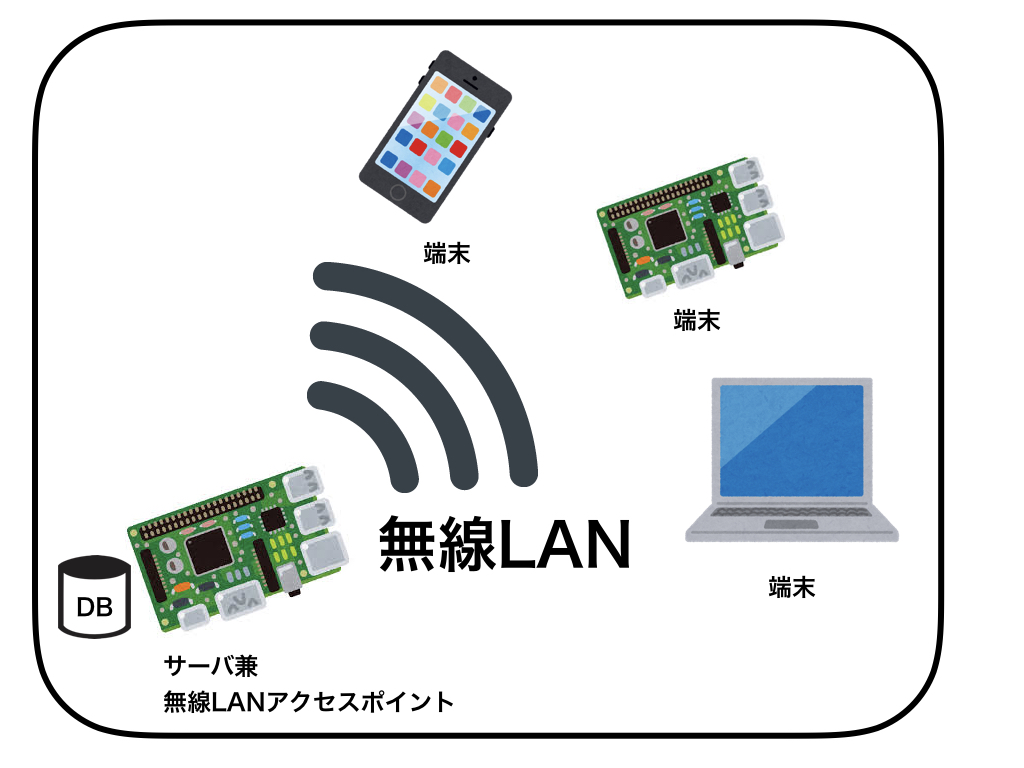
\includegraphics[width=1\linewidth,clip]{./img/wifi.jpeg}
    \caption{ログイン画面のイメージ図}\label{fig:wifi}
  \end{center}
\end{figure}
